% ----------------------------------------------------
% Literature Review
% ----------------------------------------------------
\documentclass[class=report,11pt,crop=false]{standalone}
% Page geometry
\usepackage[a4paper,margin=20mm,top=25mm,bottom=25mm]{geometry}

% Font choice
\usepackage{lmodern}

\usepackage{lipsum}

% Use IEEE bibliography style
\bibliographystyle{IEEEtran}

% Line spacing
\usepackage{setspace}
\setstretch{1.20}

% Ensure UTF8 encoding
\usepackage[utf8]{inputenc}

% Language standard (not too important)
\usepackage[english]{babel}

% Skip a line in between paragraphs
\usepackage{parskip}

% For the creation of dummy text
\usepackage{blindtext}

% Math
\usepackage{amsmath}

% Header & Footer stuff
\usepackage{fancyhdr}
\pagestyle{fancy}
\fancyhead{}
\fancyhead[R]{\nouppercase{\rightmark}}
\fancyfoot{}
\fancyfoot[C]{\thepage}
\renewcommand{\headrulewidth}{0.0pt}
\renewcommand{\footrulewidth}{0.0pt}
\setlength{\headheight}{13.6pt}

% Epigraphs
\usepackage{epigraph}
\setlength\epigraphrule{0pt}
\setlength{\epigraphwidth}{0.65\textwidth}

% Colour
\usepackage{color}
\usepackage[usenames,dvipsnames]{xcolor}

% Hyperlinks & References
\usepackage{hyperref}
\definecolor{linkColour}{RGB}{77,71,179}
\hypersetup{
    colorlinks=true,
    linkcolor=linkColour,
    filecolor=linkColour,
    urlcolor=linkColour,
    citecolor=linkColour,
}
\urlstyle{same}

% Automatically correct front-side quotes
\usepackage[autostyle=false, style=ukenglish]{csquotes}
\MakeOuterQuote{"}

% Graphics
\usepackage{graphicx}
\graphicspath{{Images/}{../Images/}}
\usepackage{makecell}
\usepackage{transparent}

% SI units
\usepackage{siunitx}

% Microtype goodness
\usepackage{microtype}

% Listings
\usepackage[T1]{fontenc}
\usepackage{listings}
\usepackage[scaled=0.8]{DejaVuSansMono}

% Custom colours for listings
\definecolor{backgroundColour}{RGB}{250,250,250}
\definecolor{commentColour}{RGB}{73, 175, 102}
\definecolor{identifierColour}{RGB}{196, 19, 66}
\definecolor{stringColour}{RGB}{252, 156, 30}
\definecolor{keywordColour}{RGB}{50, 38, 224}
\definecolor{lineNumbersColour}{RGB}{127,127,127}
\lstset{
  language=Matlab,
  captionpos=b,
  aboveskip=15pt,belowskip=10pt,
  backgroundcolor=\color{backgroundColour},
  basicstyle=\ttfamily,%\footnotesize,        % the size of the fonts that are used for the code
  breakatwhitespace=false,         % sets if automatic breaks should only happen at whitespace
  breaklines=true,                 % sets automatic line breaking
  postbreak=\mbox{\textcolor{red}{$\hookrightarrow$}\space},
  commentstyle=\color{commentColour},    % comment style
  identifierstyle=\color{identifierColour},
  stringstyle=\color{stringColour},
   keywordstyle=\color{keywordColour},       % keyword style
  %escapeinside={\%*}{*)},          % if you want to add LaTeX within your code
  extendedchars=true,              % lets you use non-ASCII characters; for 8-bits encodings only, does not work with UTF-8
  frame=single,	                   % adds a frame around the code
  keepspaces=true,                 % keeps spaces in text, useful for keeping indentation of code (possibly needs columns=flexible)
  morekeywords={*,...},            % if you want to add more keywords to the set
  numbers=left,                    % where to put the line-numbers; possible values are (none, left, right)
  numbersep=5pt,                   % how far the line-numbers are from the code
  numberstyle=\tiny\color{lineNumbersColour}, % the style that is used for the line-numbers
  rulecolor=\color{black},         % if not set, the frame-color may be changed on line-breaks within not-black text (e.g. comments (green here))
  showspaces=false,                % show spaces everywhere adding particular underscores; it overrides 'showstringspaces'
  showstringspaces=false,          % underline spaces within strings only
  showtabs=false,                  % show tabs within strings adding particular underscores
  stepnumber=1,                    % the step between two line-numbers. If it's 1, each line will be numbered
  tabsize=2,	                   % sets default tabsize to 2 spaces
  %title=\lstname                   % show the filename of files included with \lstinputlisting; also try caption instead of title
}

% Caption stuff
\usepackage[hypcap=true, justification=centering]{caption}
\usepackage{subcaption}

% Glossary package
% \usepackage[acronym]{glossaries}
\usepackage{glossaries-extra}
\setabbreviationstyle[acronym]{long-short}

% For Proofs & Theorems
\usepackage{amsthm}

% Maths symbols
\usepackage{amssymb}
\usepackage{mathrsfs}
\usepackage{mathtools}

% For algorithms
\usepackage[]{algorithm2e}

% Spacing stuff
\setlength{\abovecaptionskip}{5pt plus 3pt minus 2pt}
\setlength{\belowcaptionskip}{5pt plus 3pt minus 2pt}
\setlength{\textfloatsep}{10pt plus 3pt minus 2pt}
\setlength{\intextsep}{15pt plus 3pt minus 2pt}

% For aligning footnotes at bottom of page, instead of hugging text
\usepackage[bottom]{footmisc}

% Add LoF, Bib, etc. to ToC
\usepackage[nottoc]{tocbibind}

% SI
\usepackage{siunitx}

% For removing some whitespace in Chapter headings etc
\usepackage{etoolbox}
\makeatletter
\patchcmd{\@makechapterhead}{\vspace*{50\p@}}{\vspace*{-10pt}}{}{}%
\patchcmd{\@makeschapterhead}{\vspace*{50\p@}}{\vspace*{-10pt}}{}{}%
\makeatother
\makenoidxglossaries

\newacronym{radar}{RADAR}{Radio Detection and Ranging}
\usepackage{graphicx} % for including images

\begin{document}
\ifstandalone
\tableofcontents
\fi
% ----------------------------------------------------
\chapter{Literature Review \label{ch:literature}}
%\epigraph{If you wish to make an apple pie from scratch, you must first invent the universe.}%
%    {\emph{---Carl Sagan}}
\vspace{-0.5cm}
% ----------------------------------------------------
\section{Power Solutions for Remote Camera Traps}
Powering camera traps in remote environments like the Kalahari Desert presents unique challenges due to limited access to grid power. Traditional battery-powered setups are impractical due to maintenance needs and limited lifespan. Therefore, alternative power sources, such as solar energy, are crucial for sustained functionality.

\subsection{Solar-Powered Camera Systems for Remote Monitoring}
Solar-powered camera traps offer a sustainable solution, utilizing abundant sunlight to operate autonomously, without relying on grid power or frequent battery replacements. Research on solar-powered systems, like in Reference \cite{PowerNestingRaptors}, demonstrates their effectiveness in wildlife monitoring. These systems employ solar panels to power cameras, antennas, and batteries, ensuring continuous operation even in remote areas. Additionally, projects like "SlugCam" \cite{OutdoorVideoMonitoring} focus on optimizing power consumption for prolonged battery life. On-board current sensing allows these systems to adapt operation based on available battery charge levels, enhancing efficiency and reliability.

\subsection{Storage Method For Excess Energy}
To enhance solar power systems, one can incorporate a battery for power storage. The battery is designed to store any excess electricity generated by solar panels, ensuring efficient utilization of solar energy and continuous operation when there is no solar power \cite{Palmetto}. Storage solutions are integral to solar-powered camera traps. These batteries provide backup power during periods of low sunlight, ensuring continuous operation.

Lithium-ion (Li-ion) batteries are the most popular form of solar batteries currently on the market \cite{Palmetto}. "Solar panel companies prefer lithium-ion batteries because they can store more energy, hold that energy longer than other batteries, and have a higher \acrfull{DoD}" \cite{Palmetto}. Lithium batteries are much more expensive than their lead-acid counterparts but are an effective way to drastically reduce the size and weight of a video system \cite{CAMDevelopmentOfNestMonitoring}.

Lead batteries can last for days on a single charge, with recharging taking approximately 3 hours of sunlight \cite{PowerNestingRaptors}. While lead batteries are still available at affordable prices, their popularity is declining due to their low \acrshort{DoD} and relatively shorter lifespan compared to other battery technologies \cite{Palmetto}. 

From the above, this combination of solar power and efficient energy storage enables camera traps to function reliably in remote environments like the Kalahari Desert.

\newpage
\section{Efficient Computing Systems for Low-Cost Remote Monitoring
}
In recent years, there has been significant advancement in microprocessor and microcontroller-based systems, providing cost-effective solutions for developing smart devices and streamlining the automotive process. With their unprecedented levels of performance, efficiency and versatility, these systems have become invaluable tools for many various projects. These systems have gained traction as promising tools in low-cost remote monitoring, offering affordable solutions for ornithologists. 

\subsection{Selection of Low-Powered microcontrollers}

In remote bird monitoring, where environmental conditions and resource constraints pose significant challenges, the selection of an appropriate micro-processing platform is paramount to the effective operation of the monitoring system. Studies have highlighted the Arduino, ESP32, and Raspberry Pi as popular choices for remote monitoring systems, citing their versatility and suitability for diverse monitoring requirements \cite{ArduinoCCTV} \cite{ESP32Design} \cite{RaspSys}. %  Each of these platforms offers unique features and capabilities, making them well-suited for different monitoring applications. %

\textbf{Arduino} 

Founded as an open-source hardware and software initiative in 2005, the Arduino has since become synonymous with user-friendliness, offering hobbyists and novice programmers an accessible platform for \acrfull{DIY} projects \cite{systemArduino} \cite{ArduinoCCTV}.

The Arduino platform offers seamless interfacing through its dedicated Arduino \acrfull{IDE} and supports the widely acclaimed C/C++ syntax \cite{systemArduino}.  C/C++ is considered as a low level programming language, and well known for it's efficiency, especially for microcontrollers. Though low-level programming can be quite complex, the Arduino \acrshort{IDE} uses a simplified version of C, making project development accessible to novice developers \cite{PerformanceC++} \cite{systemArduino}.  This accessibility is further enhanced by the inclusion of  extensive documentation and a large support community \cite{systemArduino}. User-friendly microcontrollers, such as those offered by the Arduino platform, simplify the development process for remote monitoring systems, allowing for focus on implementing the necessary sensing, data transmission, and data processing functionalities without the hindrance of complex programming or hardware setup procedures. 

Reference \cite{systemArduino}  describes the Arduino as cost-effective and dependable. Their dependability can be seen by the numerous  fields they are applied in; fields including health care, agriculture,  home automation and the mining industry \cite{systemArduino} \cite{ArduinoCCTV}. 

Among the array of strengths highlighted, Reference \cite{systemArduino} reveals that the microcontrollers' most compelling feature lies in its "consumption of very low power consumption." This low power consumption is particularly advantageous for remote monitoring applications, as it allows these systems to operate for extended periods without the need for frequent battery replacements or recharging.

\textbf{ESP32}

Despite its small profile with dimensions ($25.5mm \times 18.0mm \times 2.8mm$), the ESP32 stands as a formidable piece of hardware. Introduced in 2016, this microcontroller was purposefully crafted for robust functionality in \acrfull{IOT} application development \cite{ESP32Design}. A distinguishing trait of the ESP32 is its integrated Wi-Fi and Bluetooth capabilities, making it an indispensable asset for projects reliant on wireless communication, particularly those involving remote monitoring \cite{ESPComp}. 

Similarly to the Arduino, the ESP32 can be interfaced with, using the Arduino \acrshort{IDE} and programmed with C/C++ and the Arduino's simplified version. \cite{ESPComp}. As a result, the ESP32 inherits the user-friendliness and simplicity that comes with the Arduino, the extensive documentation and the large support community in conjunction with its own set of documentation and support community. 

The ESP32's key strength lies in its exceptionally low power consumption, much like the Arduino. As noted in Reference \cite{ESP32Design}, the ESP32 achieves remarkable efficiency through the incorporation and integration of "sleep modes and power management features." The incorporation of sleep modes proves invaluable for remote monitoring applications, allowing systems to conserve power and extend their operating lifespan.

\textbf{Raspberry Pi}

The Raspberry Pi, though technically cannot be classified as a microcontroller, plays a pivotal role in \acrshort{IOT} applications. It is regarded as a \acrfull{SBC} or micro-computer due to having computer-like performance and features, within a small form factor \cite{RaspSys}. This \acrshort{SBC} boasts a variety of versions, each with varying IO capabilities. However, they all share fundamental features such as: an integrated Linux Operating System, integrated support for microSD storage, Wi-Fi, Bluetooth, and an HDMI port for display output \cite{RaspSys}.

Despite its powerful performance and numerous computer-like features, Reference \cite{RaspSys} mentions, the Raspberry Pi manages to maintain its affordability and ease of use. Supporting a \acrfull{GUI} interface and the Python programming syntax, which is recognized as a "very high-level language" and offers "many sources for learning", it reinforces the narrative of simple and user-friendly programming \cite[p.~2]{PythLang}.


\subsection{Sensor Interfacing}

Sensor interfacing enables the integration of various sensors with microcontrollers for data acquisition and processing. Though there are multiple types of interfacing protocols, \acrshort{UART}, \acrshort{SPI} and \acrshort{I2C} serve as the most commonly used protocols in microcontroller development \cite{SerialEval}. 

In Reference \cite{SerialEval}, it is revealed that these protocols vary in transmission speed and power consumption, both of which are important factors for remote monitoring. Within Reference \cite{SerialEval}, we find that \acrshort{UART} supports a maximum transmission rate of $50\ \acrshort{Mbps}$. Using approximately $53\ \mu J$ of energy to transmit 9 bytes of data in $5{,}78\ mS$. In comparison to \acrshort{UART}, \acrshort{SPI} offers a faster transmission rate, achieving speeds of up to $70\ \acrshort{Mbps}$. Additionally, it consumes less energy, utilizing only $22\ \mu J$ transfer the same 9 bytes over a period of $4{,}6\ mS$. \acrshort{I2C} is not far off from \acrshort{SPI}, having a slight higher energy consumption of $31\ \mu J$, transmitting the same 9 byte data set over $5{,}91\ mS$. \acrshort{I2C}, however, does offers the slowest rate amongst \acrshort{UART} and \acrshort{SPI}, achieving speeds of up to $3{,}4\ \acrshort{Mbps}$.  

\newpage
\section{Exploring Data Transfer Methods}

\subsection{Local Host File Server}
Many microcontrollers and microcomputers have built-in Wi-Fi capabilities. An ESP32, for example, has many uses and can be connected to multiple types of devices. "An ESP32 can implement TCP/IP, full 802.11 b/g/n/e/i WLAN MAC protocol, and Wi-Fi Direct specifications" \cite[p~3]{WiFiSpecs}.  These specifications allow them to run local host web file servers.

ESP32 Microcontrollers and many others act in three connection modes which are Access Point, Wi-Fi Station, or a combination of both \cite{WiFiConnections}. Access Point allows for other devices to connect to the microcontroller over its built-in Wi-Fi transmitter. This feature is used to connect to the microcontrollers local network.

The frequency of their transmitters/receivers is 2.4GHz which is suitable to download files over Wi-Fi from a web server \cite{WiFiSpecs}.

Using a web page file with a ".html" extension, a file server page can be created, and by running web-server code, the microcontroller can be connected to via its IP address when connected to its Wi-Fi access point \cite{WiFiSpecs}.

Using the web-page, a front-end interface is created where a device that is connected to the microcontroller’s local host website can view the files on it. Here the connected device can choose to download (or manage) the files of the microcontroller. The web-page can also be configured to monitor other data from the microcontroller/microcomputer such as sensor data and relay it back visually.

\subsection{Bluetooth}
Bluetooth technology uses radio waves to transmit data. In most cases Bluetooth can be quite power intensive, however there is a version of Bluetooth that is known for being energy efficient.  \acrfull{BLE} is an optimized version of Bluetooth which is made to use less power than other energy-saving technologies \cite{BLE_Info}. However, a major short fall is that it has a maximum transfer speed of approximately 1 \acrshort{Mbps} \cite{BLE_Web}.

Bluetooth on devices that utilise \acrshort{BLE} usually stays in sleep mode and only wakes up when activity occurs. This is called the Deep Sleep State, where the current consumption is less than $1 \mu A$, and it replaces the "idle mode" of traditional Bluetooth \cite{BLE_Specs}. This works by only communicating for a few seconds between the master and slave and then it returns to its sleep state.

In addition to the deep sleep state another method that \acrshort{BLE} uses to reduce power consumption is its reduction in the number of broadcasting bands. Instead of the 16-32 bands that conventional Bluetooth uses \acrshort{BLE} only uses 3 \cite{BLE_Specs}.

\newpage
\section{Exploring Methodologies and Considerations in Bird Camera Footage Capture}

Camera footage was first used in ornithological research over 50 years ago \cite{CAMFirst} and "camera technology has been used with increasing frequency between 1956 and 2007" \cite[p.~190]{CAMDevelopmentOfNestMonitoring}. 
Automatically gathering camera footage of birds is essential as "such technology allows for the collection of data that would otherwise be impractical to obtain" \cite[p.~186]{CAMDevelopmentOfNestMonitoring} as well as the footage "provide[s] researchers with glimpses of extremely rare events or unknown behavior" \cite[p.~186]{CAMDevelopmentOfNestMonitoring}. 

There are multiple different methods and variations of camera footage capture. The main differences in methodologies are how often the footage is captured, day time versus night time capture and the focal length of the camera.

\subsection{Frequency of Camera Footage Capture}

A variety of different footage capture frequencies are used in ornithological research which range from continuous video to still pictures. Each method has its own strengths and weaknesses including, but not limited to, which research topics it can and can not be applied to and its cost.

The most common method of footage capture in ornithological research was to use time-lapse video systems that record at between 2 and 25 \acrfull{fps} \cite{CAMDevelopmentOfNestMonitoring}. This method was mostly use to track predators of birds' nests \cite{CAMDevelopmentOfNestMonitoring} where the time lapse footage had the advantage of using less storage and power while still enabling researchers to identify the predators by family or species $63\%$ of the time \cite{CAMTimeLapsePredators}. According to Reference \cite{CAMTimeLapsePredators}, the main hindrance for the identification of species was the definition of the compressed image. 

The second most common method was still picture capturing that used manual or infra-red triggers \cite{CAMDevelopmentOfNestMonitoring} \cite{CAMBirdCollisions}. These systems were only able to be used for nest predator identification and feeding ecology, but they were also the preferred method for those investigations \cite{CAMDevelopmentOfNestMonitoring} \cite{CAMRemoteWildlifePhotography}. 

The third most common method was to use continuous real time footage capture and this method was mainly used for behavioural studies \cite{CAMDevelopmentOfNestMonitoring}. Interestingly, most implementations of real time footage capture did not capture footage continuously for 24 hours of the day, but rather 2 to 4 hour periods where about half of these systems had an inbuilt trigger  while some others were manually activated \cite{CAMDevelopmentOfNestMonitoring}. The systems that  captured footage for 24 hours of the day were reportedly easier to setup and use \cite{CAMDVR24hr} and some used \acrlong{AI} to filter the footage into usable data and/or clips \cite{CAMAIModels}.

A few studies took a slight alteration to real time footage where they captured short videos ($<30s$) using a trigger system. These studies mainly looked at the behaviour of bird that did not remain in the same location for very long \cite{CAMInexpensiveRPVideo} \cite{CAMBirdCollisions}. 

\subsection{Day time versus night time footage}

During the day time in minimally shaded areas, visual light is sufficient to capture footage with, however some studies required footage during the night for nocturnal species and sometimes for diurnal species. Several studies have shown that artificial visible light at night has a substantial negative effect on birds' migration, breeding activities, feeding habits and behaviour \cite{CAMNightLights1} \cite{CAMNightLights2} \cite{CAMNightLights3} \cite{CAMNightLightsRed}. 

Most studies that required footage of birds during the low light hours of dusk, dawn and night used infra red light to capture their images \cite{CAMDevelopmentOfNestMonitoring} \cite{CAMIRCam} \cite{CAMIRCamComparrisson}. Interestingly, while it has been found that birds have four cones in their eyes which allows them to see into the ultraviolet spectra \cite{CAMBirdSeeNoIR} \cite{CAMBirdSeeUV}, they are still unable to detect \acrfull{IR} light \cite{CAMBirdSeeNoIR}. Further studies augment this information with the facts that visible red light does significantly affect birds \cite{CAMNightLightsRed} and that their boundary for \acrshort{IR} light is similar to that of a human's \cite{CAMBirdSeeNoIR} which is about $700 nm$ \cite{CAMHumanIRLimit}. 

While birds do emit a small amount of \acrlong{IR} and \acrlong{NIR} light \cite{CAMBirdEmitIR}, studies have shown that augmenting the image capture with simple \acrshort{IR} \acrshort{LEDs} allows for successful footage capture which is highly reliable compared to other methods of bird detection at night time \cite{CAMIRCamComparrisson} \cite{CAMIRCam}. Another study further specifies that \acrshort{IR} light with shorter wave lengths of around $850 nm$ provided better footage in minimal light conditions \cite{CAMDevelopmentOfNestMonitoring}

\subsection{Focal Length and Aperture of a Camera} 

The focal length and aperture of a camera are related to depth of field of the camera where a lower focal length and a smaller aperture give a higher depth of field or, in other words, a larger area where the camera will be focused \cite{CAMFOV1} \cite{CAMFOV2}. A study suggested that if it is possible to place the camera close to the bird ($\leq 2m$), a wide angle lens ($\leq 8 mm$ focal length) was sufficient \cite{CAMDevelopmentOfNestMonitoring}.

\subsection{Costs of various implementations of camera}

Cameras, video and time lapse capturing devices for bird can vary in cost dramatically. High end, commercial devices can be over a few thousand dollars \cite{CAMInexpensiveVideo}, however "custom-built Raspberry Pi cameras are increasingly popular research tools in the fields of behavioral ecology and conservation" \cite[p.~14585]{CAMInexpensiveRPVideo}. Reference \cite{CAMInexpensiveRPVideo} was able to create a triggered video capture system for around \$133 per unit which were able to achieve a 70\% success rate with 138 deployments. The majority of failures of these devices were reportedly caused by humidity, overheating or a dislodged connection. 

\newpage
\section{Camera Triggering Methods: Sensors for Effective Camera Trapping}

Camera triggering activates a camera to capture data in response to specific conditions or events. A camera trap's function is straightforward: it waits in the field until an animal passes by, then automatically captures an image or video, storing the data for later analysis \cite{HowCamersTrapsWork}. 

Object detection sensors play a crucial role in triggering cameras where sensors can be in the form of motion detection, heat detection, sound detection, and image recognition. Different types of sensors offer distinct advantages and drawbacks, but sensor fusion can be employed to combine their information which compensates for each others' limitations, and provides comprehensive data \cite{ImageUltrasonicFusion}.

The success of camera traps hinges on their proper setup, ensuring that animals move across the detection zone rather than towards or away from the camera \cite{HowCamersTrapsWork}. An effective sensor triggering mechanism should possess several key attributes, including ease of implementation, responsiveness, reliability, adjustable sensitivity, and real-time feedback. These features facilitate seamless integration with monitoring systems and ensure prompt and accurate detection of events or activities.


\subsection{Understanding Different Footage Capture Technologies}
\acrfull{PIR} sensors are widely favoured for motion detection in camera trapping, primarily due to their affordability, energy efficiency, and high reliability \cite{CommonMisconceptions}.  These sensors are triggered upon detecting a sudden change in heat energy, usually prompted by the movement of an animal. They achieve this by sensing the electromagnetic radiation emitted from objects in their vicinity. 

\acrfull{mmWave} radar operates by transmitting high-frequency electromagnetic waves and receiving their reflections from objects in the surrounding environment. These reflections are then utilized to detect and localize objects with high accuracy \cite{mmWave1}. An ultrasonic sensor, which has similar functionality to \acrshort{mmWave} sensors, emits a pulse of ultrasonic waves towards a target and calculates distance measurement based on the elapsed time between the emission of the wave and the reception of the echo \cite{UltrasonicAgri} \cite{UltrasonicObjectDetect}. Acoustic sensors, without emitting any signal to the target, serve to detect sounds and convert them into electrical signals. The real challenge in object detection using acoustic sensors lies in processing the incoming signal.

\acrfull{IBD} systems include the use of cameras, along with machine learning algorithms, to detect objects. Typically, \acrshort{IBD} systems work in conjunction with \acrfull{MBD} systems, which are commonly employed for indoor localization and tracking, utilizing smart floors, tiles, and carpets to detect human footsteps through structural vibration \cite{ShutteredPIR}.



\subsection{Comparing Sensor Performance and Features}

The intensity of radiation reaching the \acrshort{PIR} sensors is influenced by the medium through which the electromagnetic radiation propagates. Therefore, the accuracy of \acrshort{PIR} sensor readings may be affected by the quality of the surrounding air \cite{CommonMisconceptions}. Reference \cite{HowCamersTrapsWork} found that “gradual temperature changes, such as clouds passing across the sun, do not generate enough localized temperature difference to make the \acrshort{PIR} trigger the camera.” 

\acrshort{mmWave} technology offers several advantages, including low-light functionality, cost-effectiveness, and the ability to penetrate small objects using "5G-and-beyond devices." Typically, \acrshort{mmWave} technology offers longer detection ranges compared to PIR sensors, often up to several meters. This makes it an ideal choice for outdoor object detection and has led to its increasing popularity in autonomous vehicles \cite{mmWave3}. \acrshort{mmWave} sensors are less prone to false alarms caused by environmental factors like wind-blown vegetation or changes in ambient temperature. Generally, \acrshort{mmWave} sensors consume more power compared to \acrshort{PIR} sensors, especially if operating continuously \cite{mmWavePower}.

Typically, an ultrasonic distance sensor comprises an element that produces sound and a microphone that captures the reflected echo. The strength of the reflected wave is determined by the shape, composition, and orientation of an object \cite{UltrasonicAgri}. 

In a study by Reference \cite{AcousticSensing}, the feasibility of using bird songs for object detection and classification to safeguard agricultural goods from bird attacks was explored. This system comprises a sensor module deployed in the field and a cloud-based software unit. Initially, the sensor module conducts pre-filtering to assess the likelihood of a critical bird species being present in the area. If specific sound patterns or behaviours indicative of the target bird species are detected, the sensor module initiates the second phase of processing.

During the second phase, the sensor module transmits relevant audio data, such as bird songs via a cloud-based software. This software unit utilizes machine learning algorithms for the dependable recognition and classification of the transmitted audio data. While the second phase is more accurate and reliable in identifying bird species compared to the first phase, it requires additional computational resources \cite{AcousticSensing}.

\begin{figure}[h]
    \centering
    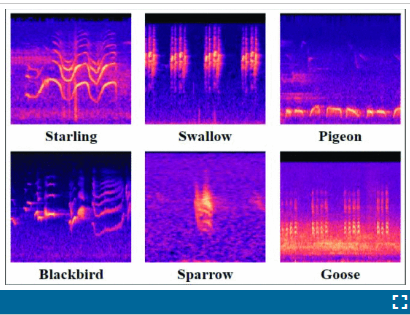
\includegraphics[width=0.6\textwidth]{AcousticSensing [11].png}
    \caption{Bird Song Differentiation – 6 Different Species \cite{AcousticSensing}}
    \label{fig:birdsounds}
\end{figure}

Once the target bird has been identified, the cloud-based system can remotely trigger appropriate actions to protect the crops, showcasing its potential application for camera traps \cite{AcousticSensing}.

\subsection{Challenges and Limitations of Camera Trap Systems}
Reference \cite{ShutteredPIR} noted that \acrshort{PIR} sensors are motion detectors by nature and fail to detect static objects in an environment. In Reference \cite{HowCamersTrapsWork}, it was highlighted that the \acrshort{PIR} sensor's functionality is affected by certain shortcomings. Specifically, smaller targets present challenges in detection as they emit less heat, while distant targets are also harder to detect because the heat they emit reaches the detector in lesser amounts. The Kalahari’s elevated temperature, paired with the detection range which diminishes when a hot background reduces the temperature contrast between the background and the target, could result in missed opportunities to capture footage of birds. Reference \cite{HowCamersTrapsWork} found that “If the camera itself gets hot enough, and it can do if it is in the sun, the \acrshort{PIR} sensor is blinded by being hotter than both the animals and the background, and it will not trigger at all until it has cooled down, which may take a few hours and lead to missed images until well after dusk.”

Textured objects, fur, or wool can absorb much of the sound wave emitted by the ultrasonic sensor so that very little is reflected back to the sensor. In testing conducted by Reference \cite{UltrasonicAgri}, ultrasonic sensors were evaluated for their ability to detect objects commonly found in outdoor agricultural environments, including a Dracaena plant, a dog model, and a wood fence post. It was observed that objects with extremely soft surface textures, such as the dog model, could go undetected at any distance from the sensor. Similarly, Reference \cite{UltrasonicObjectDetect} conducted a similar test using a rippled cloth and found that the sound waves were not efficiently reflected. These findings suggest that objects with a soft exterior, such as birds, may potentially go completely unnoticed by an ultrasonic sensor.

\acrfull{IBD} systems suffer degraded performance under adverse conditions (poor illumination) \cite{mmWave4}. The \acrshort{IBD} systems face drawbacks due to the need of light, sensor position, and complicated signal processing procedures. The \acrshort{IBD} systems are often complemented with other sensors, such as \acrshort{mmWave} or \acrshort{PIR}, to improve its performance.

For ornithological purposes, \acrshort{MBD} systems are not desirable. While one might contemplate installing such a system beneath a bird's nest to trigger a camera, the natural environment presents numerous sources of vibration, leading to a high likelihood of false triggers. Additionally, birds are relatively lightweight, necessitating a high sensitivity level in the system, which introduces a new set of challenges. Moreover, \acrshort{MBD} systems require significant maintenance to ensure optimal functionality.

One significant drawback of acoustic sensors is their reliance on a continuous internet connection to facilitate real-time data transmission for timely detection. This necessity imposes a requirement for consistent connectivity, which can be challenging in remote or off-grid locations \cite{AcousticSensing}. Furthermore, utilizing high-end microphones for accurate acoustic sensing might result in cost inefficiencies, given their relatively expensive procurement and maintenance requirements.

\newpage
\section{Exploring Methods for Non-Invasive Bird Temperature Monitoring}
There are multiple methods of measuring temperature of birds all with varying levels of effectiveness and invasiveness to the bird. Internal temperature via thermometry involves capturing a bird and inserting a rectal thermometer to read the temperature. While this method is simple, ‘the stress of capture and indeed the temperature measurement itself can bring about stress-induced hyperthermia’ \cite{TEMPMeasuringChallenges} which negatively affects both the bird and the accuracy of the measurement.

There are two alternative, remote methods of capturing internal temperature data. The first is to use a surgically implanted device that would log the temperature and could be retrieved at a later date. The second method had the bird ingest a gastrointestinal device in the form of a pill that would pass through the birds digestive track, gathering data as it travelled. Interestingly, a study found that the ‘retention time [of the pill] was actually improved by increasing the size of the device’ \cite{TEMPMeasuringChallenges}.

Both of these methods posed a challenge in retrieving the data from the device once it has run out of battery or been discharged from the bird. Reference \cite{TEMPMeasuringChallenges} proposed a solution to each of these problems. Adding a telemetry system to the surgically implanted device, it could transmit its data to a ground station that could be stationed near to where the bird frequents. As for the gastrointestinal pill, the bird could be strapped with a telemetry receiver station that would communicate with a  telemetry-enabled pill; this strapped on telemetry receiver which could be more easily retrieved.

Lastly, external body temperature can be read remotely and non-invasively using infra- red radiation sensors. This method would be easier to implement as no capture of the bird is required. Interestingly, multiple studies have shown that internal body temperature strongly relates to eye and external skin temperature \cite{TEMPMeasuringChallenges} \cite{TEMPSkinSurface} \cite{TEMPThermalImaging} \cite{TEMPBodySurface} however, it relates weakly to plumage temperature \cite{TEMPBodySurface}. This is shown in the figure below. Thus, the infra-red sensor would either have to have a high resolution or be able to be targeted at the bird's exposed skin or eye. 

\begin{figure}[h]
    \centering
    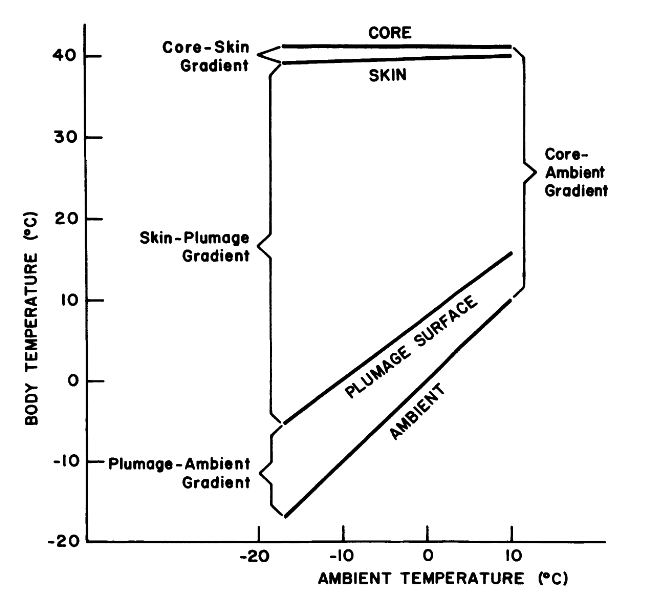
\includegraphics[width=0.4\textwidth]{BodyTemp.png}
    \caption{Temperature of different measurement sites versus ambient temperature \cite{TEMPBodySurface}}
    \label{fig:temprelations}
\end{figure}

% ----------------------------------------------------
\ifstandalone
\bibliography{../Bibliography/References.bib}
\printnoidxglossary[type=\acronymtype,nonumberlist]
\fi
\end{document}
% ----------------------------------------------------